\documentclass{article}

% Workshop track: double-blind (OpenReview).
% If the workshop confirms single-blind, switch to: \usepackage[sglblindworkshop]{neurips_2026}
\usepackage[dblblindworkshop]{neurips_2026}

% Workshop title appears in the footer of each page.
\workshoptitle{SocialAgent: Second Workshop on Large Language Models for Social Reasoning and Simulation}

\usepackage[utf8]{inputenc}
\usepackage[T1]{fontenc}
\usepackage{hyperref}
\usepackage{url}
\usepackage{booktabs}
\usepackage{amsfonts}
\usepackage{nicefrac}
\usepackage{microtype}
\usepackage{xcolor}
\usepackage{graphicx}
\usepackage{amsmath}
\usepackage{multirow}

% Figures are in the same directory as this file
\graphicspath{{./}}

\title{Moral Judgment or Framing Artifact? A Process Dissociation Analysis of\\
27 Frontier LLMs Across Moral Foundations}

% Omit for double-blind review
\author{Anonymous}

\begin{document}

\maketitle

% ============================================================================
\begin{abstract}
% ============================================================================

Large language models (LLMs) are increasingly deployed as social agents and proxies for human moral reasoners in simulations—yet whether their moral judgments reflect genuine deliberation or sensitivity to surface framing remains unknown. We apply the Conway and Gawronski (2013) process dissociation paradigm to 27 frontier LLMs, administering 80 moral dilemmas organized across five moral foundations (Care, Fairness, Loyalty, Authority, Purity) and eight real-world domains in both congruent (no utilitarian justification; both frameworks oppose harm) and incongruent (utilitarian justification conflicts with deontological prohibition) variants, with $n = 50$ independent trials per model. The \emph{moral sensitivity gap}—incongruent minus congruent harm endorsement rate—quantifies susceptibility to utilitarian framing. All 26 capable models substantially exceed the human moral sensitivity gap (human: 30.70 pp; model mean: 56.71 pp, SD = 5.45 pp), a systematic excess of $+$26 pp. Critically, extended chain-of-thought reasoning does not reduce this susceptibility: in 6 of 8 matched within-lab pairs, reasoning models produce equal or larger gaps than their non-reasoning counterparts, and a group-level test finds no significant advantage for non-reasoning models (Welch's $t(25) = 1.618$, $p = 0.119$, $d = 0.56$). Foundation-level analysis reveals a 53 pp spread from the most susceptible domain (Loyalty: 76.05 pp) to the least (Care: 23.26 pp)—the latter falling \emph{below} the human baseline, suggesting RLHF-specific suppression of harm in care contexts. These findings challenge the use of frontier LLMs as valid moral reasoning proxies in social simulations and introduce the process dissociation paradigm as a principled evaluation tool for social agents.

\end{abstract}

% ============================================================================
\section{Introduction}
% ============================================================================

As LLMs are integrated into multi-agent systems, social simulations, and interactive decision environments, a foundational question arises: do these models engage in genuine moral reasoning, or do their moral outputs primarily reflect framing effects inherited from training? The distinction carries practical consequences. An LLM that tracks the moral structure of a situation—weighing obligations, rights, and consequences—is qualitatively different from one whose outputs are determined by how a situation is rhetorically framed. The latter would be unreliable as a moral agent and potentially dangerous in deployed systems, since adversarial or incidental variations in framing could produce radically different moral outputs from the same underlying situation.

Existing alignment work has focused on preventing overtly harmful outputs through reinforcement learning from human feedback \citep{ouyang2022training} and Constitutional AI \citep{bai2022constitutional}. While effective at reducing surface harmful behaviors, these methods do not guarantee coherent moral reasoning across framing contexts. A model may refuse a direct request to harm while endorsing the same harm when framed as instrumentally necessary—a pattern with direct implications for adversarial prompting, value manipulation, and the use of LLMs as agents with moral authority.

Empirical work on LLM moral judgment has primarily used accuracy-based ethics benchmarks \citep{hendrycks2021aligning, scherrer2024evaluating}, simplified trolley-problem variants, or survey instruments drawn from moral psychology \citep{abdulhai2023moral}. These approaches assess what models say about morality but do not cleanly separate genuine moral reasoning from framing susceptibility. No prior work has applied paradigms designed specifically to decompose these components at a scale covering the breadth of current frontier models.

We address this gap by adapting the process dissociation paradigm of \citet{conway2013deontological}—a method from moral psychology designed to independently estimate deontological and utilitarian response tendencies—to a battery of 80 moral dilemmas spanning five moral foundations \citep{graham2009liberals} and eight real-world domains. We apply this paradigm to 27 frontier LLMs in the most comprehensive behavioral moral evaluation of this kind to date, covering models from 12 organizations across four countries and including both standard autoregressive and extended chain-of-thought reasoning variants.

Our main contributions are: (1) evidence that all capable frontier LLMs substantially and consistently exceed the human moral sensitivity gap, pointing to systematic framing susceptibility; (2) within-lab reasoning contrasts showing that extended chain-of-thought deliberation does not reduce susceptibility and in most cases increases it; (3) foundation-level analysis revealing dramatic heterogeneity in framing susceptibility across moral domains, including a reversal of expected human patterns in the Care foundation; and (4) a demonstration that the process dissociation paradigm provides a principled diagnostic tool for evaluating moral cognition in LLM-based social agents.

% ============================================================================
\section{Related Work}
% ============================================================================

\paragraph{The process dissociation paradigm.}
\citet{conway2013deontological} introduced a method for separately estimating deontological and utilitarian response tendencies from moral dilemma data. \emph{Congruent} dilemmas pit both frameworks against endorsing harm, establishing a baseline harm-aversion rate; \emph{incongruent} dilemmas introduce a strong utilitarian justification that conflicts with deontological prohibition, measuring susceptibility to consequentialist override. The \emph{moral sensitivity gap}—endorsement in incongruent minus congruent conditions—quantifies this susceptibility as a continuous individual-difference measure. Human participants in \citet{conway2013deontological} showed a gap of 30.70 pp (congruent: 25.38\%, incongruent: 56.08\%), which serves as our comparison benchmark. This framework is distinct from simple trolley-problem variants \citep{foot1967problem, thomson1985trolley} and from dual-process accounts of moral judgment \citep{greene2001fmri, cushman2013action} in that it produces a within-subject decomposition rather than treating one scenario as a proxy for a moral system. Crucially, it operationalizes \emph{framing susceptibility} rather than treating it as a confound to be controlled.

\paragraph{Moral Foundations Theory.}
Haidt's Moral Foundations Theory \citep{haidt2001emotional, graham2009liberals} posits five distinct moral foundations—Care, Fairness, Loyalty, Authority, Purity—reflecting evolved psychological systems that vary across individuals and cultures. Prior work applying MFT to LLMs \citep{abdulhai2023moral} used questionnaire-based methods assessing stated moral values. We extend this tradition behaviorally: rather than asking what models say about moral foundations, we measure how their judgment differs across them in a controlled behavioral paradigm.

\paragraph{LLMs in social simulations.}
LLMs are increasingly used as synthetic participants in social simulations and agent-based models \citep{park2023generative}, and in large-scale moral experiments \citep{awad2018moral}. These applications implicitly assume that LLM moral outputs are valid proxies for human moral reasoning. Our results bear directly on this assumption. The Moral Machine experiment \citep{awad2018moral} demonstrated large-scale human moral variation; a key open question is whether LLMs replicate this variation or produce systematically different patterns.

\paragraph{LLM moral evaluation.}
The ETHICS benchmark \citep{hendrycks2021aligning} and subsequent work \citep{scherrer2024evaluating} have established that LLMs show differential performance across moral domains and sensitivity to presentation format. However, accuracy-based benchmarks measure compliance with a ground truth rather than the structure of moral reasoning. Our paradigm measures framing susceptibility—a behavioral property that accuracy metrics cannot assess—and applies it at a scale ($n = 27$ models, $n = 50$ trials each) that permits cross-model generalization.

% ============================================================================
\section{Methods}
% ============================================================================

\subsection{Stimulus Set}

We constructed 80 moral dilemmas in a $5 \times 8 \times 2$ factorial design: five moral foundations $\times$ eight real-world domains (economic, historical, law enforcement, medical, military, personal, scientific research, transportation) $\times$ two variants (congruent, incongruent). Each dilemma placed the model in the first-person role of the moral actor and asked three questions: (1) \textbf{harm endorsement} (primary DV): \emph{Is the described action appropriate?} (Yes/No); (2) \textbf{likelihood}: \emph{How likely would you be to take this action?} (1--7); (3) \textbf{confidence}: \emph{How confident are you?} (1--7). We report harm endorsement throughout.

Congruent variants presented situations where harm lacked compelling justification, aligning both deontological prohibition and utilitarian calculus against endorsement. Incongruent variants added a strong utilitarian argument for the same harmful action (e.g., causing harm to one to prevent greater harm to many). Dilemma pairs were structurally parallel—differing only in the presence and framing of the utilitarian justification—so the gap in endorsement across variants is directly attributable to susceptibility to that framing.

\subsection{Models and Procedure}

We tested 27 frontier LLMs (Table~\ref{tab:results}) accessed via the OpenRouter API, spanning 12 organizations across the USA, China, France, South Korea, and Canada. Models were classified as \emph{reasoning} (extended chain-of-thought; $n = 8$) or \emph{non-reasoning} (standard autoregressive; $n = 19$). Reasoning models included o1, o3, Claude Opus 4, Grok 3, Gemini 2.5 Pro, DeepSeek R1, DeepSeek R1-0528, and Qwen3 235B (Thinking), enabling within-lab contrasts for six lab families.

Each model received all 80 dilemmas in randomized order (seed fixed at 42 for reproducibility) across $n = 50$ independent runs at temperature 1.0 to sample natural response variability. Non-reasoning models received a 150-token maximum; reasoning models received 3{,}000 tokens with a 300-second timeout. Responses were parsed with a multi-stage procedure stripping markdown formatting, chain-of-thought tags (\texttt{<think>...</think>}), numbered-list prefixes, and bracket echoing. Trials with missing or unparseable responses were excluded from analysis. One model (GPT-4o-mini) was run at $n = 10$ due to resource constraints and is treated as preliminary.

\subsection{Primary Measure}

The \textbf{moral sensitivity gap} = incongruent harm endorsement \% $-$ congruent harm endorsement \% is our primary outcome. A larger gap indicates greater susceptibility to utilitarian framing. All comparisons reference the human baseline of 30.70 pp from \citet{conway2013deontological}.

% ============================================================================
\section{Results}
% ============================================================================

\subsection{Universal Excess Over the Human Gap}

Table~\ref{tab:results} reports harm endorsement rates and moral sensitivity gaps for all 27 models. The most striking result is unambiguous: \emph{all 26 capable models substantially exceed the human moral sensitivity gap}. Human participants show a gap of 30.70 pp; model gaps range from 45.70 pp (Solar Pro 3) to 65.78 pp (Claude 3.5 Sonnet), with a mean of 56.71 pp (SD = 5.45 pp) across models with $n = 50$—a mean excess of $+$26.01 pp. Figure~\ref{fig:overall} shows all 27 models sorted by gap.

\begin{table}[t]
\centering
\caption{Harm endorsement rates and moral sensitivity gaps for all 27 models ($n = 50$ per model unless noted). \textbf{R} = reasoning model (extended chain-of-thought). Human baseline from \citet{conway2013deontological}. Llama 3.2 3B shows a capacity failure and is excluded from group analyses (see text).}
\label{tab:results}
\small
\begin{tabular}{lcccc}
\toprule
\textbf{Model} & \textbf{R} & \textbf{Congruent \%} & \textbf{Incongruent \%} & \textbf{Gap (pp)} \\
\midrule
Claude 3.5 Sonnet       &   & 25.64 & 91.42 & 65.78 \\
Llama 4 Maverick        &   & 20.80 & 85.90 & 65.10 \\
o3                      & Y & 22.25 & 86.70 & 64.45 \\
Gemini 2.5 Pro          & Y & 27.46 & 91.75 & 64.29 \\
Mixtral 8x22B           &   & 15.15 & 77.00 & 61.85 \\
Grok 3                  & Y & 23.65 & 84.95 & 61.30 \\
Grok 4                  &   & 21.90 & 82.10 & 60.20 \\
DeepSeek R1             & Y & 17.94 & 78.11 & 60.17 \\
GPT-5                   &   & 24.95 & 84.80 & 59.85 \\
Qwen3 235B              &   & 17.49 & 76.55 & 59.06 \\
Ernie 4.5               &   & 19.40 & 76.85 & 57.45 \\
DeepSeek R1-0528        & Y & 16.17 & 73.61 & 57.44 \\
GPT-3.5 Turbo           &   & 23.35 & 80.60 & 57.25 \\
Gemma 3 27B             &   & 22.25 & 78.90 & 56.65 \\
o1                      & Y & 22.85 & 78.17 & 55.32 \\
Claude Opus 4           & Y & 17.95 & 72.26 & 54.31 \\
Command A               &   & 19.49 & 73.20 & 53.71 \\
Mistral Large 3         &   & 28.30 & 81.90 & 53.60 \\
GPT-4o                  &   & 21.35 & 74.90 & 53.55 \\
DeepSeek V3             &   & 21.69 & 74.69 & 53.00 \\
Qwen3 235B (Thinking)   & Y & 14.02 & 66.56 & 52.54 \\
Nova Premier            &   & 17.71 & 68.77 & 51.05 \\
Phi-4                   &   & 24.68 & 73.97 & 49.29 \\
Llama 3.3 70B           &   & 32.39 & 78.77 & 46.38 \\
Solar Pro 3             &   &  9.12 & 54.82 & 45.70 \\
GPT-4o-mini$^\dagger$   &   & 20.00 & 75.25 & 55.25 \\
Llama 3.2 3B$^\ddagger$ &   &  3.23 &  0.00 & $-$3.23 \\
\midrule
Human (C\&G 2013)       &   & 25.38 & 56.08 & 30.70 \\
\bottomrule
\multicolumn{5}{l}{\small $^\dagger$ Preliminary: $n = 10$ only.
  \quad $^\ddagger$ Capacity failure; excluded from group analyses.}
\end{tabular}
\end{table}

\begin{figure}[t]
  \centering
  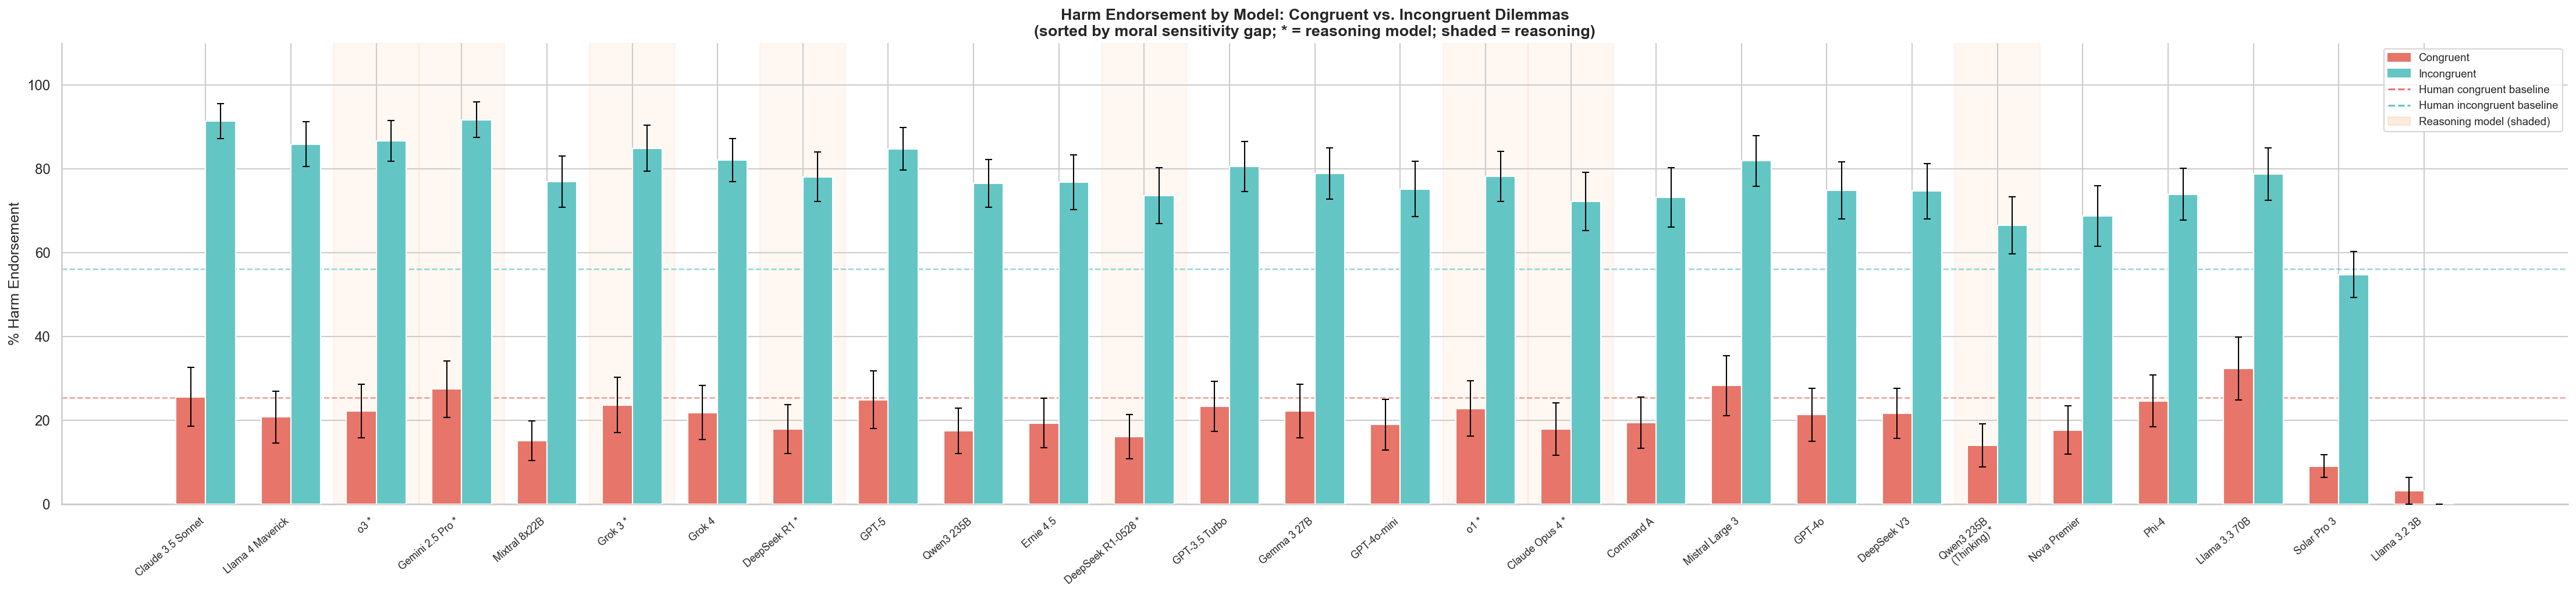
\includegraphics[width=\linewidth]{overall_chart.png}
  \caption{Harm endorsement rates (coral = congruent; teal = incongruent) for all 27 tested models, sorted by moral sensitivity gap. Dashed lines mark the human baseline from \citet{conway2013deontological}. Shaded columns indicate reasoning models. Every capable model exceeds the human gap.}
  \label{fig:overall}
\end{figure}

An important decomposition reveals where cross-model variation originates. Congruent endorsement rates are relatively stable across models (range: 9.1\%--32.4\%), clustering near the human congruent baseline of 25.38\%. By contrast, incongruent endorsement shows dramatic variation (54.8\%--91.8\%), far above the human incongruent rate of 56.08\%. Virtually all cross-model variation in the gap is thus attributable to differential susceptibility to utilitarian framing, not to differences in baseline harm aversion.

Two models merit special note. \textbf{Solar Pro 3} (Upstage, South Korea) is the only model whose incongruent endorsement (54.82\%) falls below the human incongruent baseline (56.08\%)—a qualitatively different profile that warrants further investigation and may reflect cultural or institutional training differences. \textbf{Llama 3.2 3B} shows near-zero endorsement in both conditions (congruent: 3.23\%, incongruent: 0.00\%) and a negative gap ($-3.23$ pp), indicating that at this parameter scale the model lacks the capacity for the structured moral reasoning required by this task; it is excluded from all group-level analyses.

\subsection{Extended Chain-of-Thought Reasoning Does Not Reduce Framing Susceptibility}

A critical question for social agent design is whether reasoning models—which engage in explicit deliberation before responding—show lower framing susceptibility than standard models. Our results consistently argue against this. Figure~\ref{fig:withinlab} shows within-lab contrasts for 8 matched pairs.

\begin{figure}[t]
  \centering
  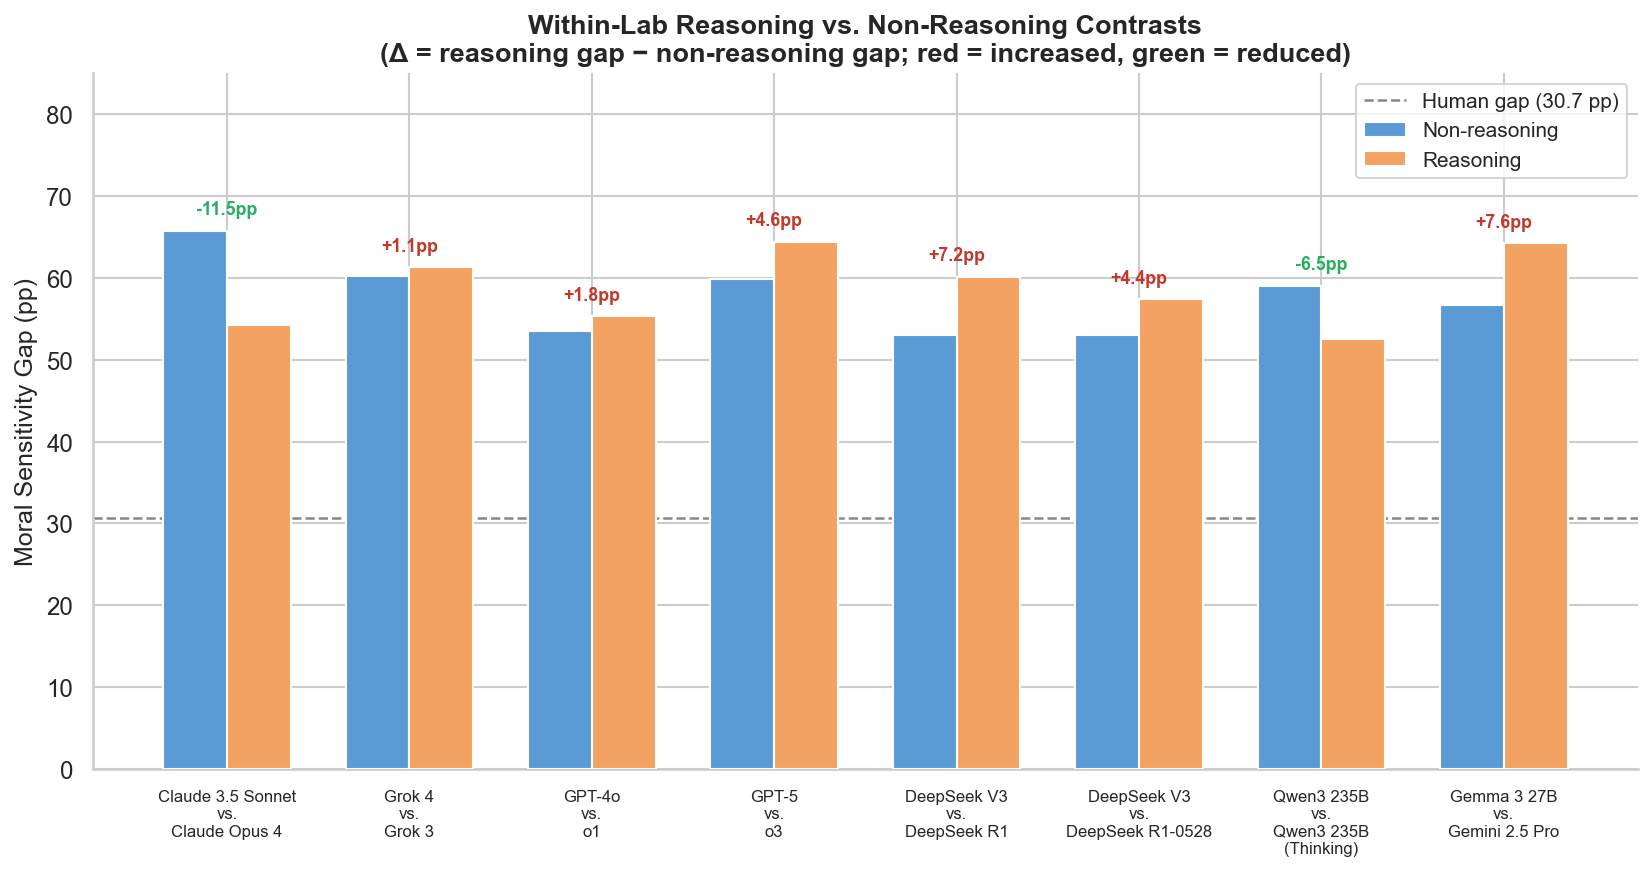
\includegraphics[width=\linewidth]{within_lab_contrasts.png}
  \caption{Within-lab reasoning vs.\ non-reasoning contrasts. Blue bars show the moral sensitivity gap for the non-reasoning model; orange bars for the matched reasoning model. Annotated $\Delta$ values = reasoning $-$ non-reasoning gap; red = reasoning is more susceptible; green = reasoning is less susceptible. Dashed line marks the human baseline (30.70 pp).}
  \label{fig:withinlab}
\end{figure}

In 6 of 8 within-lab pairs, the reasoning model produces an equal or \emph{larger} gap than its non-reasoning counterpart:
\begin{itemize}
  \item xAI: Grok 3 vs.\ Grok 4 ($\Delta = +1.10$ pp)
  \item OpenAI: o1 vs.\ GPT-4o ($\Delta = +1.77$ pp)
  \item OpenAI: o3 vs.\ GPT-5 ($\Delta = +4.60$ pp)
  \item DeepSeek: R1 vs.\ V3 ($\Delta = +7.17$ pp)
  \item DeepSeek: R1-0528 vs.\ V3 ($\Delta = +4.44$ pp)
  \item Google: Gemini 2.5 Pro vs.\ Gemma 3 27B ($\Delta = +7.64$ pp)
\end{itemize}
Only two labs show reasoning \emph{reducing} the gap: Anthropic (Claude Opus 4 vs.\ Claude 3.5 Sonnet: $\Delta = -11.47$ pp) and Qwen (Qwen3 235B Thinking vs.\ Standard: $\Delta = -6.52$ pp).

A group-level Welch's $t$-test confirms no significant benefit for non-reasoning models. Reasoning models ($M = 58.73$ pp, $SD = 4.53$, $n = 8$) trend \emph{higher} than non-reasoning models ($M = 52.71$ pp, $SD = 14.64$, $n = 19$), with a non-significant difference ($t(25) = 1.618$, $p = 0.119$, Cohen's $d = 0.56$). The wide non-reasoning SD reflects genuine between-family heterogeneity rather than a systematic effect of reasoning. This finding holds even when the $d$ value is noted: the effect size would favor reasoning models being \emph{more} susceptible, not less, though the difference is not reliable at this sample size.

\subsection{Foundation-Level Heterogeneity: Loyalty and Fairness Drive the Gap}

Figure~\ref{fig:foundations} shows the moral sensitivity gap pooled across all capable models by moral foundation. The pattern reveals substantial heterogeneity spanning 52.79 pp:

\begin{itemize}
  \item \textbf{Loyalty}: $M = 76.05$ pp (SE = 1.75)
  \item \textbf{Fairness}: $M = 75.25$ pp (SE = 2.99)
  \item \textbf{Authority}: $M = 69.63$ pp (SE = 1.29)
  \item \textbf{Purity}: $M = 39.19$ pp (SE = 2.88)
  \item \textbf{Care}: $M = 23.26$ pp (SE = 2.65)
\end{itemize}

\begin{figure}[t]
  \centering
  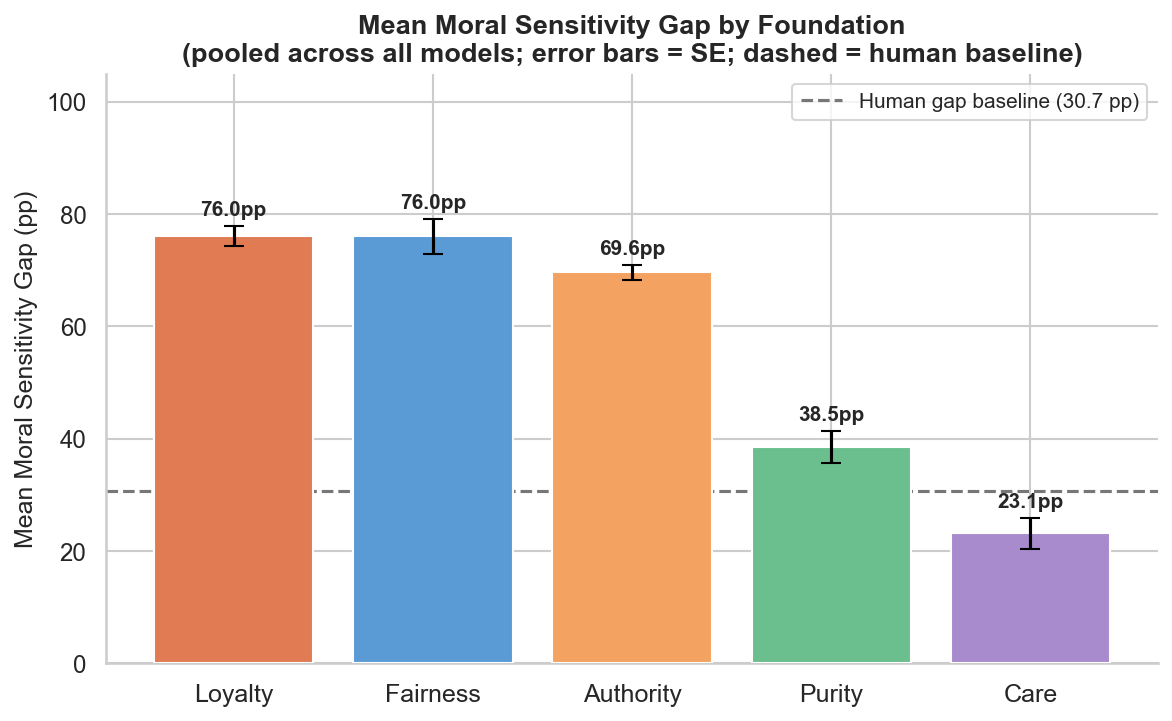
\includegraphics[width=0.9\linewidth]{foundation_gaps.png}
  \caption{Mean moral sensitivity gap by moral foundation, pooled across all capable models (error bars = SE across models). The dashed line marks the human gap baseline (30.70 pp). Loyalty and Fairness show the largest framing susceptibility; Care falls \emph{below} the human baseline, suggesting RLHF-driven suppression.}
  \label{fig:foundations}
\end{figure}

In Loyalty and Fairness dilemmas, models near-universally endorse harm when a utilitarian justification is provided, suggesting almost complete susceptibility to framing override in these domains. The Care result is the most striking departure: at 23.26 pp, LLMs are \emph{less} susceptible to utilitarian framing in Care contexts than the human baseline of 30.70 pp. Classic trolley-problem scenarios—arguably the most studied moral dilemmas—are Care scenarios, and human participants typically show substantial framing effects there \citep{foot1967problem, greene2001fmri}. The LLM inversion of this pattern—lowest susceptibility precisely where humans show prominent effects—likely reflects RLHF-based training that specifically suppresses harm endorsement in harm/care contexts, given their prevalence in human feedback datasets. Purity (39.19 pp) is above the human baseline but substantially lower than Loyalty, Fairness, and Authority, partially consistent with findings that purity-based moral intuitions show some resistance to consequentialist override in humans \citep{haidt2001emotional}.

% ============================================================================
\section{Discussion}
% ============================================================================

\paragraph{Framing susceptibility over genuine deliberation.}
The central pattern across all three analyses is difficult to reconcile with an account in which LLMs engage in genuine moral deliberation. If models were reasoning carefully about costs and benefits, we would expect: (a) moral sensitivity gaps calibrated near the human level; (b) reasoning models showing \emph{reduced} susceptibility through explicit deliberation; and (c) some convergence across model families as a function of shared moral content. Instead we observe: (a) a systematic $+$26 pp excess over human gaps; (b) reasoning models trending \emph{higher} than non-reasoning models; and (c) substantial between-family variation (SD = 5.45 pp) not explained by reasoning type, scale, or organizational origin.

A more parsimonious account is that LLM moral outputs primarily reflect training-induced distributional patterns—specifically, a tendency to endorse rhetorically salient utilitarian arguments. The process dissociation paradigm cleanly isolates this: the incongruent condition provides such an argument, and models show near-universal endorsement far exceeding the human rate. The congruent rates, by contrast, cluster near human levels, indicating that baseline harm aversion is roughly calibrated; it is the susceptibility to consequentialist override that is dramatically out of range. This is consistent with \citet{scherrer2024evaluating}'s finding that LLM moral outputs are sensitive to presentation format, and with broader evidence that LLMs respond to surface properties of prompts rather than their deeper semantic structure.

\paragraph{Implications for social simulation validity.}
A growing literature uses LLMs as proxies for human participants in social simulations \citep{park2023generative} and moral experiments \citep{awad2018moral}. Our findings suggest this practice requires substantial caution when moral reasoning is involved. LLMs do not replicate human moral sensitivity patterns at the aggregate level (they are uniformly over-susceptible) or at the foundation level (the Care/human baseline inversion suggests a qualitatively different response profile). A social simulation substituting LLM moral agents for human ones risks producing systematically misleading results, particularly in Loyalty and Fairness domains where LLM susceptibility is highest. The present paradigm provides a diagnostic tool for calibrating and validating LLM moral behavior before such substitution.

\paragraph{The Anthropic exception.}
The one consistent case where reasoning reduced framing susceptibility was Claude Opus 4 vs.\ Claude 3.5 Sonnet ($\Delta = -11.47$ pp)—the largest reduction in our dataset. The Qwen family also shows a reduction ($\Delta = -6.52$ pp). These exceptions suggest that the relationship between reasoning and framing susceptibility is not uniform and may depend on training philosophy. Constitutional AI \citep{bai2022constitutional}, which involves explicit moral principles, may interact with chain-of-thought reasoning in ways that reduce rather than increase framing sensitivity. Identifying the specific mechanisms is an important direction for future work.

\paragraph{Limitations.}
Several limitations apply. First, our sample is a snapshot of models available as of mid-2025 and may not generalize to subsequent model generations. Second, harm endorsement in a structured text survey may not reflect how models would behave as decision-making agents in interactive, real-world-like settings; a planned second study in a Minecraft-based simulation environment will assess whether these text-based patterns replicate in embodied contexts. Third, a high moral sensitivity gap could in principle reflect appropriate moral sensitivity (correctly weighing consequences) rather than susceptibility to framing, though the systematic excess of $+$26 pp above human rates and the reasoning finding together make this interpretation less tenable. Fourth, GPT-4o-mini ($n = 10$) is preliminary; we include it for completeness but do not draw conclusions from it.

% ============================================================================
\section{Conclusion}
% ============================================================================

We present the most comprehensive behavioral evaluation of LLM moral judgment to date, applying the process dissociation paradigm to 27 frontier models across five moral foundations and eight real-world domains. Every capable model substantially exceeds the human moral sensitivity gap, pointing to systematic framing susceptibility rather than calibrated moral deliberation. Extended chain-of-thought reasoning does not resolve this: in 6 of 8 within-lab contrasts, reasoning models show equal or larger gaps than their non-reasoning counterparts. Foundation-level analysis reveals a 53 pp spread from Care (most resistant; uniquely below the human baseline) to Loyalty (most susceptible), with a Care inversion that likely reflects RLHF-driven suppression of harm endorsement in harm/care contexts. Together, these findings challenge the validity of frontier LLMs as moral reasoning proxies in social simulations and propose the process dissociation paradigm as a principled diagnostic framework for evaluating moral cognition in LLM-based social agents.

\begin{ack}
Omitted for anonymous review.
\end{ack}

\bibliographystyle{plainnat}
\bibliography{references}

\end{document}
